\documentclass[12pt,a4paper]{article}
\usepackage{amsmath, amssymb, geometry, booktabs, xcolor, hyperref,
            listings, pgfplots, tcolorbox, enumitem, fancyhdr, tikz, array}
\usepgfplotslibrary{fillbetween}
\geometry{margin=2.5cm}
\pgfplotsset{compat=1.18}
\tcbuselibrary{skins, breakable}

% Define custom environments
\newtcolorbox{curiositybox}[1]{colback=yellow!10, colframe=orange!80, title=#1, breakable}
\newtcolorbox{infobox}[1]{colback=blue!5, colframe=blue!60, title=#1, breakable}
\newtcolorbox{mistakebox}[1]{colback=red!5, colframe=red!60, title=#1, breakable}
\newtcolorbox{learnbox}[1]{colback=green!5, colframe=green!60, title=#1, breakable}

% Header and Footer
\pagestyle{fancy}
\fancyhf{}
\lhead{Special Matrices}
\rhead{Unit 2 -- LAC}
\cfoot{\thepage}

% Document Title Setup
\title{\textbf{Special Matrices} \\ \large Unit 2 -- Eigenvalues, Eigenvectors, Diagonalization and Quadratic Forms}
\author{Department of Mathematics}
\date{\today}

\begin{document}
\maketitle
\tableofcontents
\newpage

%============================================================
\section{Real-World Engineering Hook}
%============================================================

\begin{curiositybox}{Why Should an Engineer Care?}
Consider a robotics arm performing a pick-and-place operation on an assembly line.
Every rotation of that arm in 3D space is encoded by an \textbf{orthogonal matrix} $Q$ satisfying $Q^\top Q = I$.
Because $\det(Q) = \pm 1$, the rotation preserves lengths and angles perfectly --- no distortion, no stretch, no shear.
Lose the orthogonality property and your robot arm crushes the component instead of placing it.

In \textbf{quantum mechanics}, every measurable physical quantity (energy, momentum, spin) is represented by a \textbf{Hermitian operator} $A = A^H$.
The eigenvalues of $A$ are always real, which is physically necessary: you cannot measure an imaginary energy level.
The entire framework of quantum computing relies on unitary matrices ($U^H U = I$) to represent reversible quantum gates that preserve probability.

In \textbf{machine learning and statistics}, least-squares regression computes the \textbf{projection matrix} $P = A(A^\top A)^{-1}A^\top$,
which is both symmetric ($P^\top = P$) and idempotent ($P^2 = P$).
Applying the projection twice gives the same result as applying it once --- exactly what ``projection'' should mean geometrically.
These are not abstract curiosities; they are the structural guarantees that make engineering algorithms reliable.
\end{curiositybox}

%============================================================
\section{Why This Topic Exists}
%============================================================

The five special matrix families studied here are not an arbitrary zoo of definitions.
Each family emerges from a geometric or physical constraint, and each constraint produces exactly the eigenvalue behaviour an engineer needs.

\vspace{0.5em}
\begin{center}
\begin{tabular}{@{}lll@{}}
\toprule
\textbf{Matrix Type} & \textbf{Defining Property} & \textbf{Engineering Consequence} \\
\midrule
Symmetric \& Skew-Symmetric & $A = A^\top$ or $A = -A^\top$ & Real eigenvalues for FEM stiffness matrices \\
Orthogonal & $Q^\top Q = I$ & Rigid-body rotations preserve norms \\
Hermitian \& Skew-Hermitian & $A = A^H$ or $A = -A^H$ & Real measurables in quantum circuits \\
Idempotent \& Nilpotent & $A^2 = A$ or $A^k = 0$ & Projection operators; nilpotent shift registers \\
Unitary \& Normal & $U^H U = I$; $AA^H = A^H A$ & Quantum gates; spectral theorem for complex matrices \\
\bottomrule
\end{tabular}
\end{center}

\vspace{1em}
\begin{learnbox}{Core Learning Objectives}
By the end of this topic, a student should be able to:
\begin{itemize}
  \item State the defining equation of each of the five special matrix families.
  \item Verify whether a given real or complex matrix belongs to a special class.
  \item State and apply the eigenvalue constraints for each class.
  \item Construct the projection matrix from a column vector and verify idempotency.
  \item Distinguish between orthogonal (real) and unitary (complex) matrices.
\end{itemize}
\end{learnbox}

%============================================================
\section{Intuition First \& Mathematical Definitions}
%============================================================

\subsection{Symmetric and Skew-Symmetric Matrices}

Imagine folding a square matrix along its main diagonal.
If the matrix looks identical after the fold, it is \emph{symmetric}.
If every entry flips its sign, it is \emph{skew-symmetric}.
Symmetric matrices arise naturally in physical systems where the interaction between component $i$ and component $j$ equals the interaction between $j$ and $i$---think of the stiffness matrix in structural analysis.

\begin{infobox}{Symmetric and Skew-Symmetric Matrices: Definitions and Properties}
\textbf{Symmetric Matrix:}
A square matrix $A \in \mathbb{R}^{n \times n}$ is symmetric if
\[
  A = A^\top \quad \Longleftrightarrow \quad a_{ij} = a_{ji} \text{ for all } i,j.
\]

\textbf{Skew-Symmetric Matrix:}
$A$ is skew-symmetric if
\[
  A = -A^\top \quad \Longleftrightarrow \quad a_{ij} = -a_{ji},\quad a_{ii} = 0.
\]

\textbf{Key Properties:}
\begin{itemize}
  \item \textbf{Eigenvalues:} All eigenvalues of a real symmetric matrix are \emph{real}. All eigenvalues of a real skew-symmetric matrix are either \emph{zero or purely imaginary} (of the form $i\beta$, $\beta \in \mathbb{R}$).
  \item \textbf{Decomposition:} Any square matrix $M$ decomposes uniquely as $M = S + K$ where $S = \tfrac{1}{2}(M + M^\top)$ (symmetric) and $K = \tfrac{1}{2}(M - M^\top)$ (skew-symmetric).
  \item \textbf{Spectral Theorem:} A real symmetric matrix is orthogonally diagonalizable: $A = Q\Lambda Q^\top$ where $Q$ is orthogonal and $\Lambda$ is real diagonal.
  \item \textbf{Quadratic Form:} A symmetric matrix $A$ defines a quadratic form $\mathbf{x}^\top A \mathbf{x}$, which is real for all real $\mathbf{x}$.
\end{itemize}
\end{infobox}

\textbf{Worked Example:} Let
\[
  A = \begin{pmatrix} 3 & -1 \\ -1 & 3 \end{pmatrix}, \qquad
  B = \begin{pmatrix} 0 & 2 & -5 \\ -2 & 0 & 4 \\ 5 & -4 & 0 \end{pmatrix}.
\]
\begin{enumerate}
  \item \textbf{Verify $A$ is symmetric:} Compute $A^\top$:
    \[
      A^\top = \begin{pmatrix} 3 & -1 \\ -1 & 3 \end{pmatrix} = A. \quad \checkmark
    \]
  \item \textbf{Verify $B$ is skew-symmetric:} Compute $B^\top$:
    \[
      B^\top = \begin{pmatrix} 0 & -2 & 5 \\ 2 & 0 & -4 \\ -5 & 4 & 0 \end{pmatrix} = -B. \quad \checkmark
    \]
    Also note all diagonal entries of $B$ are $0$.
  \item \textbf{Eigenvalues of $A$:} $\det(A - \lambda I) = (3-\lambda)^2 - 1 = \lambda^2 - 6\lambda + 8 = (\lambda-2)(\lambda-4) = 0$.
    So $\lambda_1 = 2$, $\lambda_2 = 4$ --- both \emph{real}, confirming the symmetric eigenvalue theorem.
\end{enumerate}

%------------------------------------------------------------
\subsection{Orthogonal Matrices}

A rotation of a 3D rigid body does not change the length of any vector attached to the body.
The matrix that describes such a rotation is called \emph{orthogonal}: its columns form an orthonormal set,
so multiplying by it is like rotating a coordinate system without stretching or shearing.

\begin{infobox}{Orthogonal Matrices: Definitions and Properties}
\textbf{Definition:}
A real square matrix $Q \in \mathbb{R}^{n \times n}$ is \emph{orthogonal} if
\[
  Q^\top Q = I \quad \Longleftrightarrow \quad Q^\top = Q^{-1}.
\]

\textbf{Equivalent conditions:}
\begin{itemize}
  \item The columns of $Q$ form an \emph{orthonormal} basis: $\mathbf{q}_i \cdot \mathbf{q}_j = \delta_{ij}$.
  \item The rows of $Q$ also form an orthonormal basis.
\end{itemize}

\textbf{Key Properties:}
\begin{itemize}
  \item $\det(Q) = \pm 1$. ($+1$ for proper rotations; $-1$ for rotations combined with reflections.)
  \item All eigenvalues of $Q$ satisfy $|\lambda| = 1$ (they lie on the unit circle in $\mathbb{C}$).
  \item Real eigenvalues of $Q$ are restricted to $\{+1, -1\}$.
  \item Orthogonal matrices \emph{preserve norms}: $\|Q\mathbf{x}\| = \|\mathbf{x}\|$ for all $\mathbf{x}$.
  \item The inverse of an orthogonal matrix is simply its transpose: $Q^{-1} = Q^\top$.
  \item The product of two orthogonal matrices is orthogonal.
\end{itemize}
\end{infobox}

\textbf{Worked Example:} Let
\[
  Q = \begin{pmatrix} \cos\theta & -\sin\theta \\ \sin\theta & \cos\theta \end{pmatrix}
  \quad \text{(2D rotation by angle } \theta\text{)}.
\]
\textbf{Step 1. Compute $Q^\top Q$:}
\[
  Q^\top = \begin{pmatrix} \cos\theta & \sin\theta \\ -\sin\theta & \cos\theta \end{pmatrix},
\]
\[
  Q^\top Q = \begin{pmatrix} \cos\theta & \sin\theta \\ -\sin\theta & \cos\theta \end{pmatrix}
             \begin{pmatrix} \cos\theta & -\sin\theta \\ \sin\theta & \cos\theta \end{pmatrix}
           = \begin{pmatrix} \cos^2\theta + \sin^2\theta & -\cos\theta\sin\theta + \sin\theta\cos\theta \\
                             -\sin\theta\cos\theta + \cos\theta\sin\theta & \sin^2\theta + \cos^2\theta \end{pmatrix}
           = \begin{pmatrix} 1 & 0 \\ 0 & 1 \end{pmatrix} = I. \quad \checkmark
\]
\textbf{Step 2. Compute $\det(Q)$:}
$\det(Q) = \cos^2\theta + \sin^2\theta = 1$. \quad \checkmark (proper rotation)

\textbf{Step 3. Eigenvalues:}
$\det(Q - \lambda I) = (\cos\theta - \lambda)^2 + \sin^2\theta = \lambda^2 - 2\lambda\cos\theta + 1 = 0$.
$\lambda = \cos\theta \pm i\sin\theta = e^{\pm i\theta}$, so $|\lambda| = 1$. \quad \checkmark

\textbf{Specific check with $\theta = \pi/4$:}
\[
  Q_{45} = \begin{pmatrix} 1/\sqrt{2} & -1/\sqrt{2} \\ 1/\sqrt{2} & 1/\sqrt{2} \end{pmatrix}, \quad
  \det(Q_{45}) = \tfrac{1}{2} + \tfrac{1}{2} = 1. \quad \checkmark
\]
The vector $\mathbf{x} = (3, 4)^\top$ has $\|\mathbf{x}\| = 5$.
After rotation: $Q_{45}\mathbf{x} = \bigl(\tfrac{3-4}{\sqrt{2}},\, \tfrac{3+4}{\sqrt{2}}\bigr)^\top = \bigl(\tfrac{-1}{\sqrt{2}},\,\tfrac{7}{\sqrt{2}}\bigr)^\top$.
Norm $= \sqrt{\tfrac{1}{2} + \tfrac{49}{2}} = \sqrt{25} = 5$. \quad \checkmark (norm preserved)

%------------------------------------------------------------
\subsection{Hermitian and Skew-Hermitian Matrices}

When we move from real to complex matrices, the transpose $A^\top$ is replaced by the \emph{conjugate transpose} $A^H = \overline{A^\top}$.
A Hermitian matrix is the complex generalisation of a symmetric matrix.
It appears in quantum mechanics as the mathematical representation of every observable physical quantity --- position, momentum, energy --- because its eigenvalues are guaranteed to be real.

\begin{infobox}{Hermitian and Skew-Hermitian Matrices: Definitions and Properties}
Let $A \in \mathbb{C}^{n \times n}$. The \emph{conjugate transpose} is $A^H = (\bar{A})^\top$, i.e., $(A^H)_{ij} = \overline{a_{ji}}$.

\textbf{Hermitian Matrix:} $A$ is Hermitian if
\[
  A = A^H \quad \Longleftrightarrow \quad a_{ij} = \overline{a_{ji}}.
\]
Diagonal entries of a Hermitian matrix are always \emph{real} (since $a_{ii} = \overline{a_{ii}}$).

\textbf{Skew-Hermitian Matrix:} $A$ is skew-Hermitian if
\[
  A = -A^H \quad \Longleftrightarrow \quad a_{ij} = -\overline{a_{ji}}, \quad a_{ii} \in i\mathbb{R}.
\]

\textbf{Key Properties:}
\begin{itemize}
  \item All eigenvalues of a Hermitian matrix are \emph{real}.
  \item All eigenvalues of a skew-Hermitian matrix are \emph{purely imaginary or zero}.
  \item Eigenvectors corresponding to distinct eigenvalues of a Hermitian matrix are \emph{orthogonal}.
  \item A Hermitian matrix is unitarily diagonalizable: $A = U\Lambda U^H$ with $\Lambda$ real diagonal.
  \item If $A$ is real and Hermitian, then $A$ is symmetric.
  \item $A$ is Hermitian $\Longleftrightarrow$ $iA$ is skew-Hermitian.
\end{itemize}
\end{infobox}

\textbf{Worked Example:} Let
\[
  A = \begin{pmatrix} 4 & 3+i \\ 3-i & 2 \end{pmatrix}.
\]
\textbf{Step 1. Verify Hermitian:}
\[
  A^H = \overline{A^\top} = \begin{pmatrix} \overline{4} & \overline{3-i} \\ \overline{3+i} & \overline{2} \end{pmatrix}
      = \begin{pmatrix} 4 & 3+i \\ 3-i & 2 \end{pmatrix} = A. \quad \checkmark
\]
Diagonal entries $4, 2$ are real. \quad \checkmark

\textbf{Step 2. Find eigenvalues:}
\[
  \det(A - \lambda I) = (4-\lambda)(2-\lambda) - (3+i)(3-i)
    = \lambda^2 - 6\lambda + 8 - (9 + 1)
    = \lambda^2 - 6\lambda - 2.
\]
\[
  \lambda = \frac{6 \pm \sqrt{36 + 8}}{2} = \frac{6 \pm \sqrt{44}}{2} = 3 \pm \sqrt{11}.
\]
Both eigenvalues $\lambda_1 = 3 + \sqrt{11} \approx 6.317$ and $\lambda_2 = 3 - \sqrt{11} \approx -0.317$ are \emph{real}. \quad \checkmark

\textbf{Worked Example (Skew-Hermitian):} Let
\[
  B = \begin{pmatrix} 2i & 1+3i \\ -1+3i & -5i \end{pmatrix}.
\]
Check: $(B^H)_{12} = \overline{b_{21}} = \overline{-1+3i} = -1-3i$.
But $b_{12} = 1+3i \neq -(-1-3i) = 1+3i$? Re-examine:
We need $B^H = -B$, i.e., $(B^H)_{12} = -b_{12}$.
$(B^H)_{12} = \overline{b_{21}} = \overline{-1+3i} = -1-3i$ and $-b_{12} = -(1+3i) = -1-3i$. \quad \checkmark
$(B^H)_{11} = \overline{b_{11}} = \overline{2i} = -2i = -b_{11} = -2i$. \quad \checkmark
So $B$ is skew-Hermitian. Its diagonal entries $2i$ and $-5i$ are purely imaginary. \quad \checkmark

%------------------------------------------------------------
\subsection{Idempotent and Nilpotent Matrices}

When you stand in front of a mirror holding a torch, projecting the torch beam onto the mirror gives a spot of light.
Projecting that spot again onto the same mirror gives the same spot --- applying the projection twice is the same as applying it once.
That is the key property of an \emph{idempotent} matrix: $A^2 = A$.
A \emph{nilpotent} matrix, by contrast, eventually annihilates every vector: keep multiplying by $A$ and the result eventually becomes zero.

\begin{infobox}{Idempotent and Nilpotent Matrices: Definitions and Properties}
\textbf{Idempotent Matrix:} $A$ is idempotent if
\[
  A^2 = A.
\]
\textbf{Key Properties (Idempotent):}
\begin{itemize}
  \item Eigenvalues of an idempotent matrix are only $0$ or $1$.\\
    \emph{Proof:} If $A\mathbf{v} = \lambda\mathbf{v}$ then $A^2\mathbf{v} = \lambda^2\mathbf{v} = A\mathbf{v} = \lambda\mathbf{v}$, so $\lambda^2 = \lambda$, giving $\lambda \in \{0,1\}$.
  \item $\text{rank}(A) = \text{trace}(A)$.
  \item $I - A$ is also idempotent: $(I-A)^2 = I - 2A + A^2 = I - A$.
  \item $A(I - A) = A - A^2 = 0$: the column space and null space are complementary.
\end{itemize}

\textbf{Nilpotent Matrix:} $A$ is nilpotent of index $k$ if
\[
  A^k = 0 \quad \text{for some positive integer } k, \quad A^{k-1} \neq 0.
\]
\textbf{Key Properties (Nilpotent):}
\begin{itemize}
  \item All eigenvalues of a nilpotent matrix are $0$.\\
    \emph{Proof:} $A^k\mathbf{v} = \lambda^k\mathbf{v} = \mathbf{0}$ implies $\lambda = 0$.
  \item $\det(A) = 0$ (singular), $\text{trace}(A) = 0$.
  \item The characteristic polynomial of a nilpotent $n\times n$ matrix is $\lambda^n$.
\end{itemize}
\end{infobox}

\textbf{Worked Example (Idempotent):} Let
\[
  P = \begin{pmatrix} 1 & 0 & 0 \\ 0 & 0 & 0 \\ 0 & 0 & 0 \end{pmatrix}.
\]
$P^2 = P \cdot P$: the $(1,1)$ entry is $1\cdot1 + 0\cdot0 + 0\cdot0 = 1$; all other entries are $0$.
So $P^2 = P$. \quad \checkmark
Eigenvalues: $\lambda_1 = 1$ (once), $\lambda_2 = \lambda_3 = 0$ (twice). All in $\{0, 1\}$. \quad \checkmark
$\text{rank}(P) = 1 = \text{trace}(P)$. \quad \checkmark

\textbf{Worked Example (Nilpotent):} Let
\[
  N = \begin{pmatrix} 0 & 1 & 2 \\ 0 & 0 & 3 \\ 0 & 0 & 0 \end{pmatrix}.
\]
\textbf{Compute $N^2$:}
\[
  N^2 = \begin{pmatrix} 0 & 1 & 2 \\ 0 & 0 & 3 \\ 0 & 0 & 0 \end{pmatrix}
        \begin{pmatrix} 0 & 1 & 2 \\ 0 & 0 & 3 \\ 0 & 0 & 0 \end{pmatrix}
      = \begin{pmatrix} 0 & 0 & 3 \\ 0 & 0 & 0 \\ 0 & 0 & 0 \end{pmatrix}.
\]
Row 1 of $N^2$: $(0\cdot0+1\cdot0+2\cdot0,\; 0\cdot1+1\cdot0+2\cdot0,\; 0\cdot2+1\cdot3+2\cdot0) = (0,0,3)$. \quad \checkmark

\textbf{Compute $N^3$:}
\[
  N^3 = N^2 \cdot N = \begin{pmatrix} 0 & 0 & 3 \\ 0 & 0 & 0 \\ 0 & 0 & 0 \end{pmatrix}
                      \begin{pmatrix} 0 & 1 & 2 \\ 0 & 0 & 3 \\ 0 & 0 & 0 \end{pmatrix}
      = \begin{pmatrix} 0 & 0 & 0 \\ 0 & 0 & 0 \\ 0 & 0 & 0 \end{pmatrix} = 0. \quad \checkmark
\]
$N$ is nilpotent of index $k = 3$. All eigenvalues are $0$ (upper triangular with zero diagonal). \quad \checkmark

%------------------------------------------------------------
\subsection{Unitary and Normal Matrices}

A unitary matrix is the complex analogue of an orthogonal matrix.
Just as orthogonal matrices rotate real vectors without changing their lengths,
unitary matrices transform complex vectors without changing their Hermitian norms.
In quantum computing, every quantum gate that can be reversed must be unitary.
A normal matrix is the broadest class for which the spectral theorem holds in the complex setting:
any normal matrix can be diagonalized by a unitary matrix.

\begin{infobox}{Unitary and Normal Matrices: Definitions and Properties}
\textbf{Unitary Matrix:} $U \in \mathbb{C}^{n\times n}$ is unitary if
\[
  U^H U = I \quad \Longleftrightarrow \quad U^H = U^{-1}.
\]

\textbf{Key Properties (Unitary):}
\begin{itemize}
  \item $\det(U)$ satisfies $|\det(U)| = 1$.
  \item All eigenvalues of $U$ satisfy $|\lambda| = 1$.
  \item Unitary matrices preserve inner products: $\langle U\mathbf{u}, U\mathbf{v}\rangle = \langle \mathbf{u}, \mathbf{v}\rangle$.
  \item A real unitary matrix is exactly an orthogonal matrix.
  \item Every Hermitian, skew-Hermitian, and unitary matrix is normal.
\end{itemize}

\textbf{Normal Matrix:} $A \in \mathbb{C}^{n\times n}$ is normal if
\[
  AA^H = A^H A.
\]

\textbf{Key Properties (Normal):}
\begin{itemize}
  \item \textbf{Spectral Theorem (Complex):} $A$ is normal if and only if it is unitarily diagonalizable, i.e., $A = U\Lambda U^H$ for some unitary $U$ and diagonal $\Lambda$.
  \item Hermitian, skew-Hermitian, and unitary matrices are all normal.
  \item Eigenvectors of a normal matrix corresponding to distinct eigenvalues are orthogonal.
\end{itemize}
\end{infobox}

\textbf{Worked Example (Unitary):} Let
\[
  U = \frac{1}{\sqrt{2}}\begin{pmatrix} 1 & i \\ i & 1 \end{pmatrix}.
\]
\textbf{Step 1. Compute $U^H$:}
\[
  U^H = \frac{1}{\sqrt{2}}\begin{pmatrix} 1 & -i \\ -i & 1 \end{pmatrix}.
\]
\textbf{Step 2. Verify $U^H U = I$:}
\[
  U^H U = \frac{1}{2}\begin{pmatrix} 1 & -i \\ -i & 1 \end{pmatrix}\begin{pmatrix} 1 & i \\ i & 1 \end{pmatrix}
        = \frac{1}{2}\begin{pmatrix} 1\cdot1 + (-i)(i) & 1\cdot i + (-i)\cdot1 \\ (-i)\cdot1 + 1\cdot i & (-i)(i) + 1\cdot1 \end{pmatrix}.
\]
$(1,1)$: $1 + (-i)(i) = 1 - i^2 = 1 - (-1) = 2$. Multiply by $\tfrac{1}{2}$: $1$.
$(1,2)$: $i + (-i) = 0$.
$(2,1)$: $-i + i = 0$.
$(2,2)$: $(-i)(i) + 1 = 1 + 1 = 2$. Multiply by $\tfrac{1}{2}$: $1$.
\[
  U^H U = \begin{pmatrix} 1 & 0 \\ 0 & 1 \end{pmatrix} = I. \quad \checkmark
\]
\textbf{Step 3. Verify $|\det(U)| = 1$:}
\[
  \det(U) = \frac{1}{2}(1 \cdot 1 - i \cdot i) = \frac{1}{2}(1 - i^2) = \frac{1}{2}(1+1) = 1,
  \quad |\det(U)| = 1. \quad \checkmark
\]

\textbf{Worked Example (Normal):} Let
\[
  A = \begin{pmatrix} 1 & 1 \\ -1 & 1 \end{pmatrix}.
\]
$A^H = A^\top = \begin{pmatrix}1 & -1 \\ 1 & 1\end{pmatrix}$ (since $A$ is real).
\[
  AA^H = \begin{pmatrix}1&1\\-1&1\end{pmatrix}\begin{pmatrix}1&-1\\1&1\end{pmatrix}
       = \begin{pmatrix}2&0\\0&2\end{pmatrix}.
\]
\[
  A^H A = \begin{pmatrix}1&-1\\1&1\end{pmatrix}\begin{pmatrix}1&1\\-1&1\end{pmatrix}
        = \begin{pmatrix}2&0\\0&2\end{pmatrix}.
\]
$AA^H = A^H A = 2I$. \quad \checkmark \quad So $A$ is normal.

%============================================================
\section{Visual Artifacts \& Geometric Interpretation}
%============================================================

\subsection*{Diagram 1: Orthogonal Matrix Preserves the Unit Circle}

The following diagram shows that the 2D rotation matrix $Q_{45}$ maps the unit circle to itself.
Selected vectors on the unit circle are shown before rotation (blue) and after rotation (red).

\begin{center}
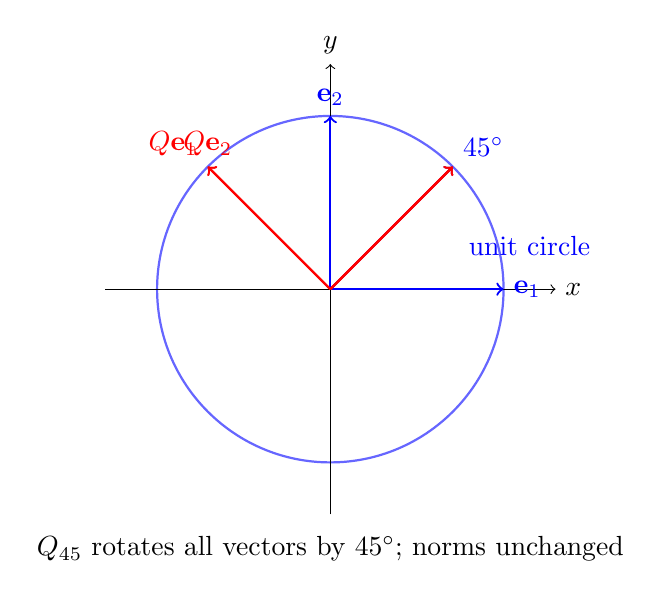
\begin{tikzpicture}[scale=2.2]
  % Unit circle
  \draw[thick, blue!60, ->] (0,0) circle (1);
  % Axes
  \draw[->] (-1.3,0) -- (1.3,0) node[right] {$x$};
  \draw[->] (0,-1.3) -- (0,1.3) node[above] {$y$};
  % Original vectors
  \draw[->, thick, blue] (0,0) -- (1,0) node[right, blue] {$\mathbf{e}_1$};
  \draw[->, thick, blue] (0,0) -- (0,1) node[above, blue] {$\mathbf{e}_2$};
  \draw[->, thick, blue] (0,0) -- ({cos(45)},{sin(45)}) node[above right, blue] {$45^\circ$};
  % Rotated vectors (by 45 degrees, so rotate by further 45)
  \draw[->, thick, red] (0,0) -- ({cos(45)},{sin(45)}) node[right, red, xshift=2pt] {};
  \draw[->, thick, red] (0,0) -- ({cos(135)},{sin(135)}) node[above left, red] {$Q\mathbf{e}_1$};
  \draw[->, thick, red] (0,0) -- ({cos(45)},{sin(45)});
  \draw[->, thick, red] (0,0) -- ({-sin(45)},{cos(45)}) node[above, red] {$Q\mathbf{e}_2$};
  % Labels
  \node[blue] at (1.15, 0.25) {unit circle};
  \node at (0,-1.5) {$Q_{45}$ rotates all vectors by $45^\circ$; norms unchanged};
\end{tikzpicture}
\end{center}

\subsection*{Diagram 2: Idempotent Matrix as Orthogonal Projection}

A projection matrix $P$ projects every vector $\mathbf{x} \in \mathbb{R}^2$ onto a line $\ell$.
Applying $P$ twice returns the same point on $\ell$ --- this is $P^2 = P$.

\begin{center}
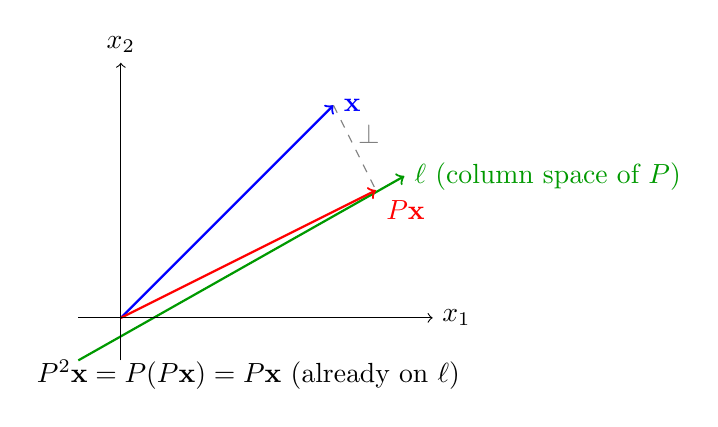
\begin{tikzpicture}[scale=1.8]
  % The line (subspace)
  \draw[thick, green!60!black, ->] (-0.3,-0.3) -- (2.0,1.0) node[right] {$\ell$ (column space of $P$)};
  % Original vector
  \draw[->, thick, blue] (0,0) -- (1.5,1.5) node[right, blue] {$\mathbf{x}$};
  % Projected vector
  \draw[->, thick, red] (0,0) -- (1.8,0.9) node[below right, red] {$P\mathbf{x}$};
  % Dashed perpendicular
  \draw[dashed, gray] (1.5,1.5) -- (1.8,0.9);
  \node[gray] at (1.75, 1.3) {$\perp$};
  % Axes
  \draw[->] (-0.3,0) -- (2.2,0) node[right] {$x_1$};
  \draw[->] (0,-0.3) -- (0,1.8) node[above] {$x_2$};
  % Note
  \node at (0.9,-0.4) {$P^2\mathbf{x} = P(P\mathbf{x}) = P\mathbf{x}$ (already on $\ell$)};
\end{tikzpicture}
\end{center}

%============================================================
\section{Step-by-Step Algorithmic Workflow}
%============================================================

\begin{infobox}{How to Verify a Special Matrix Type: Systematic Checklist}
Given a matrix $A$ (real or complex), use the following decision procedure:

\medskip
\textbf{Step 1: Compute $A^\top$ (real case) or $A^H$ (complex case).}

\medskip
\textbf{Step 2: Check symmetry / skew-symmetry (real matrices):}
\begin{itemize}
  \item If $A = A^\top$: $A$ is \textbf{symmetric}.
  \item If $A = -A^\top$: $A$ is \textbf{skew-symmetric}.
\end{itemize}

\textbf{Step 3: Check orthogonality (real matrices):}
\begin{itemize}
  \item Compute $Q^\top Q$.
  \item If $Q^\top Q = I$: $Q$ is \textbf{orthogonal}.
  \item Equivalently, check that every pair of columns satisfies $\mathbf{q}_i \cdot \mathbf{q}_j = \delta_{ij}$.
\end{itemize}

\textbf{Step 4: Check Hermitian / skew-Hermitian (complex matrices):}
\begin{itemize}
  \item If $A = A^H$: $A$ is \textbf{Hermitian}.
  \item If $A = -A^H$: $A$ is \textbf{skew-Hermitian}.
\end{itemize}

\textbf{Step 5: Check idempotency / nilpotency:}
\begin{itemize}
  \item Compute $A^2$.
  \item If $A^2 = A$: $A$ is \textbf{idempotent}.
  \item If $A^2 \neq A$, compute $A^3, A^4, \ldots$ until either $A^k = 0$ (nilpotent of index $k$) or you confirm neither.
\end{itemize}

\textbf{Step 6: Check unitary / normal (complex matrices):}
\begin{itemize}
  \item Compute $U^H U$.
  \item If $U^H U = I$: $U$ is \textbf{unitary}.
  \item Compute $AA^H$ and $A^H A$.
  \item If $AA^H = A^H A$: $A$ is \textbf{normal}.
\end{itemize}

\medskip
\textbf{Note:} A matrix may belong to multiple families simultaneously
(e.g., the identity matrix $I$ is symmetric, orthogonal, idempotent, Hermitian, unitary, and normal).
\end{infobox}

%============================================================
\section{Fully Worked Step-by-Step Numerical Examples}
%============================================================

\subsection*{Example 1: Verify a 3$\times$3 Orthogonal Matrix and Find Its Eigenvalues}

Let
\[
  Q = \begin{pmatrix}
    1 & 0 & 0 \\
    0 & 0 & -1 \\
    0 & 1 & 0
  \end{pmatrix}.
\]
This represents a $90^\circ$ rotation about the $x$-axis.

\textbf{Step 1. Compute $Q^\top$:}
\[
  Q^\top = \begin{pmatrix}
    1 & 0 & 0 \\
    0 & 0 & 1 \\
    0 & -1 & 0
  \end{pmatrix}.
\]

\textbf{Step 2. Compute $Q^\top Q$:}
\[
  Q^\top Q = \begin{pmatrix}
    1 & 0 & 0 \\
    0 & 0 & 1 \\
    0 & -1 & 0
  \end{pmatrix}
  \begin{pmatrix}
    1 & 0 & 0 \\
    0 & 0 & -1 \\
    0 & 1 & 0
  \end{pmatrix}
  = \begin{pmatrix}
    1 & 0 & 0 \\
    0 & 1 & 0 \\
    0 & 0 & 1
  \end{pmatrix} = I. \quad \checkmark
\]
Row 2 of $Q^\top$, columns of $Q$: $(0\cdot0 + 0\cdot0 + 1\cdot0,\; 0\cdot0+0\cdot0+1\cdot1,\; 0\cdot0+0\cdot(-1)+1\cdot0) = (0,1,0)$. \quad \checkmark

\textbf{Step 3. Compute $\det(Q)$:}
Expanding along row 1: $\det(Q) = 1 \cdot \det\begin{pmatrix}0&-1\\1&0\end{pmatrix} = 1 \cdot (0\cdot0 - (-1)\cdot1) = 1$. \quad \checkmark

\textbf{Step 4. Find eigenvalues:}
\[
  \det(Q - \lambda I) = \det\begin{pmatrix}
    1-\lambda & 0 & 0 \\
    0 & -\lambda & -1 \\
    0 & 1 & -\lambda
  \end{pmatrix}
  = (1-\lambda)\bigl[(-\lambda)(-\lambda) - (-1)(1)\bigr]
  = (1-\lambda)(\lambda^2 + 1).
\]
Eigenvalues: $\lambda_1 = 1$ (real), $\lambda_{2,3} = \pm i$ (modulus $1$). \quad \checkmark
All satisfy $|\lambda| = 1$, confirming orthogonality.

%-------------------------------------------------------
\subsection*{Example 2: Complex 2$\times$2 Hermitian Matrix and Its Real Eigenvalues}

Let
\[
  H = \begin{pmatrix} 5 & 2-3i \\ 2+3i & 7 \end{pmatrix}.
\]

\textbf{Step 1. Verify Hermitian:}
\[
  H^H: \quad (H^H)_{11} = \overline{5} = 5, \quad
             (H^H)_{12} = \overline{h_{21}} = \overline{2+3i} = 2-3i, \quad
             (H^H)_{21} = \overline{h_{12}} = \overline{2-3i} = 2+3i, \quad
             (H^H)_{22} = \overline{7} = 7.
\]
So $H^H = H$. \quad \checkmark Diagonal entries $5, 7$ are real.

\textbf{Step 2. Characteristic polynomial:}
\[
  \det(H - \lambda I) = (5-\lambda)(7-\lambda) - (2-3i)(2+3i).
\]
$(2-3i)(2+3i) = 4 + 9 = 13$.
$(5-\lambda)(7-\lambda) = \lambda^2 - 12\lambda + 35$.
\[
  \det(H - \lambda I) = \lambda^2 - 12\lambda + 35 - 13 = \lambda^2 - 12\lambda + 22.
\]

\textbf{Step 3. Solve $\lambda^2 - 12\lambda + 22 = 0$:}
\[
  \lambda = \frac{12 \pm \sqrt{144 - 88}}{2} = \frac{12 \pm \sqrt{56}}{2} = 6 \pm \sqrt{14}.
\]
$\lambda_1 = 6 + \sqrt{14} \approx 9.742$, $\lambda_2 = 6 - \sqrt{14} \approx 2.258$. Both \emph{real}. \quad \checkmark

%-------------------------------------------------------
\subsection*{Example 3 (Engineering): Projection Matrix in Least-Squares Regression}

In linear regression with design matrix $A = \begin{pmatrix}1\\2\\3\end{pmatrix}$ (single predictor, three observations),
the hat/projection matrix is $P = A(A^\top A)^{-1}A^\top$.

\textbf{Step 1. Compute $A^\top A$:}
$A^\top A = 1^2 + 2^2 + 3^2 = 14$.

\textbf{Step 2. Compute $(A^\top A)^{-1}$:}
$(A^\top A)^{-1} = \tfrac{1}{14}$.

\textbf{Step 3. Compute $P = A \cdot \tfrac{1}{14} \cdot A^\top$:}
\[
  P = \frac{1}{14}\begin{pmatrix}1\\2\\3\end{pmatrix}\begin{pmatrix}1&2&3\end{pmatrix}
    = \frac{1}{14}\begin{pmatrix}
        1 & 2 & 3 \\
        2 & 4 & 6 \\
        3 & 6 & 9
      \end{pmatrix}.
\]

\textbf{Step 4. Verify $P$ is symmetric ($P^\top = P$):}
$P$ is symmetric since $A(A^\top A)^{-1}A^\top$ is symmetric for any full-rank $A$. Checking entry $(1,2) = \tfrac{2}{14}$ and $(2,1) = \tfrac{2}{14}$. \quad \checkmark

\textbf{Step 5. Verify $P^2 = P$ (idempotent):}
\[
  P^2 = \frac{1}{14^2}\begin{pmatrix}1\\2\\3\end{pmatrix}
        \underbrace{\begin{pmatrix}1&2&3\end{pmatrix}\begin{pmatrix}1\\2\\3\end{pmatrix}}_{=14}
        \begin{pmatrix}1&2&3\end{pmatrix}
      = \frac{1}{14^2} \cdot 14 \cdot \begin{pmatrix}1\\2\\3\end{pmatrix}\begin{pmatrix}1&2&3\end{pmatrix}
      = \frac{1}{14}\begin{pmatrix}1\\2\\3\end{pmatrix}\begin{pmatrix}1&2&3\end{pmatrix} = P. \quad \checkmark
\]
\textbf{Engineering interpretation:} $P$ projects any response vector $\mathbf{y} \in \mathbb{R}^3$ onto the column space of $A$ (the best-fit line through the origin).
Applying $P$ twice is redundant because the projected vector already lies in the column space.

%============================================================
\section{Tabular Comparison / Workflow Reference}
%============================================================

\begin{center}
\renewcommand{\arraystretch}{1.4}
\begin{tabular}{@{}p{3.2cm} p{3.4cm} p{3.2cm} p{2.0cm} p{3.5cm}@{}}
\toprule
\textbf{Matrix Type} & \textbf{Defining Property} & \textbf{Eigenvalue Constraint} & \textbf{Inverse Formula} & \textbf{Engineering Application} \\
\midrule
Symmetric ($A \in \mathbb{R}^{n\times n}$) & $A = A^\top$ & All real & $(A^{-1})^\top = A^{-1}$ & FEM stiffness matrix, covariance matrix \\
Skew-Symmetric & $A = -A^\top$ & Zero or purely imaginary & $(-A^\top)^{-1} = -(A^{-1})^\top$ & Angular velocity (cross-product) matrix \\
Orthogonal & $Q^\top Q = I$ & $|\lambda| = 1$ & $Q^{-1} = Q^\top$ & 3D rotation, QR factorization \\
Hermitian & $A = A^H$ & All real & Standard inverse & Quantum observables, Laplacian \\
Skew-Hermitian & $A = -A^H$ & Zero or purely imaginary & Standard inverse & Quantum evolution generator \\
Idempotent & $A^2 = A$ & Only $0$ or $1$ & No inverse (singular if $A \neq I$) & Projection, regression hat matrix \\
Nilpotent (index $k$) & $A^k = 0$ & All zero & No inverse (singular) & Shift register, Jordan blocks \\
Unitary & $U^H U = I$ & $|\lambda| = 1$ & $U^{-1} = U^H$ & Quantum gates, DFT matrix \\
Normal & $AA^H = A^H A$ & Unitarily diagonalizable & Standard inverse & Spectral analysis \\
\bottomrule
\end{tabular}
\end{center}

%============================================================
\section{Common Student Mistakes \& Pitfalls}
%============================================================

\begin{mistakebox}{Frequent Errors with Special Matrices}
\begin{tabular}{@{}p{4.0cm} p{5.5cm} p{5.0cm}@{}}
\toprule
\textbf{Sub-Topic} & \textbf{Mistake} & \textbf{Correct Approach} \\
\midrule
Symmetric / Skew-Symmetric & Forgetting that skew-symmetric matrices must have all-zero diagonal entries & Check $a_{ii} = 0$ for all $i$ before declaring skew-symmetry \\
Symmetric / Skew-Symmetric & Claiming a non-square matrix can be symmetric & Symmetric/skew-symmetric are defined only for square matrices \\
Orthogonal & Confusing ``orthogonal matrix'' with ``orthogonal vectors'' & An orthogonal matrix $Q$ satisfies $Q^\top Q = I$; orthogonal vectors merely satisfy $\mathbf{u}\cdot\mathbf{v}=0$ \\
Orthogonal & Assuming det$(Q) = 1$ always & $\det(Q) = \pm 1$; reflections give $-1$ \\
Hermitian / Skew-Hermitian & Using $A^\top$ instead of $A^H$ for complex matrices & Always conjugate-transpose for complex: $A^H = \overline{A^\top}$ \\
Hermitian / Skew-Hermitian & Assuming a matrix with real entries and $A = A^\top$ is Hermitian only in the trivial sense & A real symmetric matrix is Hermitian; no complex conjugation changes anything \\
Idempotent / Nilpotent & Confusing $A^2 = A$ with $A^2 = I$ (involutory) & Idempotent: $A^2 = A$. Involutory: $A^2 = I$. These are different \\
Idempotent / Nilpotent & Assuming a nilpotent matrix has rank zero & A nilpotent matrix can have positive rank; only $A^k = 0$ for some $k$ is required \\
Unitary / Normal & Calling every diagonalizable matrix normal & A matrix is normal iff $AA^H = A^H A$; diagonalizability over $\mathbb{C}$ does not imply normality \\
Unitary / Normal & Assuming $U^H U = I$ implies $UU^H = I$ always & For square matrices they are equivalent; always verify using the square case \\
\bottomrule
\end{tabular}
\end{mistakebox}

%============================================================
\section{Comprehensive Assessment Suite}
%============================================================

\subsection*{Viva-Voce Questions}

\begin{enumerate}[label=\textbf{V\arabic*.}]
  \item \textbf{(Symmetric)} State the definition of a symmetric matrix and give two properties of its eigenvalues.
    \textit{Hint:} $A = A^\top$; eigenvalues are real; eigenvectors for distinct eigenvalues are orthogonal.
  \item \textbf{(Skew-Symmetric)} Why must every diagonal entry of a skew-symmetric matrix be zero?
    \textit{Hint:} $a_{ii} = -a_{ii}$ implies $a_{ii} = 0$.
  \item \textbf{(Orthogonal)} What is the relationship between an orthogonal matrix and its inverse?
    \textit{Hint:} $Q^{-1} = Q^\top$.
  \item \textbf{(Orthogonal)} What are the possible values of the determinant of an orthogonal matrix, and why?
    \textit{Hint:} $\det(Q^\top Q) = \det(I)$ gives $(\det Q)^2 = 1$, so $\det Q = \pm 1$.
  \item \textbf{(Hermitian)} Why are the eigenvalues of a Hermitian matrix always real, even for complex matrices?
    \textit{Hint:} If $A\mathbf{v} = \lambda\mathbf{v}$ and $A = A^H$, compute $\mathbf{v}^H A\mathbf{v}$ two ways to show $\lambda = \bar\lambda$.
  \item \textbf{(Idempotent)} If $A$ is idempotent and invertible, what must $A$ equal?
    \textit{Hint:} $A^2 = A \Rightarrow A = I$ when $A$ is invertible.
  \item \textbf{(Nilpotent)} Can a nilpotent matrix be diagonalizable (over $\mathbb{C}$)? Justify.
    \textit{Hint:} Only if it is the zero matrix; all eigenvalues are zero, and a diagonalizable nilpotent matrix $= P \cdot 0 \cdot P^{-1} = 0$.
  \item \textbf{(Unitary)} How is a unitary matrix related to an orthogonal matrix?
    \textit{Hint:} Orthogonal matrices are the real-valued special case of unitary matrices.
  \item \textbf{(Normal)} State the complex spectral theorem for normal matrices.
    \textit{Hint:} $A$ normal $\Leftrightarrow$ $A = U\Lambda U^H$ for some unitary $U$ and diagonal $\Lambda$.
  \item \textbf{(General)} Give one example of a matrix that is simultaneously symmetric, orthogonal, and idempotent.
    \textit{Hint:} The identity matrix $I$ satisfies $I = I^\top$, $I^\top I = I$, and $I^2 = I$.
\end{enumerate}

\subsection*{Descriptive Exam Questions}

\begin{enumerate}[label=\textbf{D\arabic*.}]
  \item Prove that the eigenvalues of a real skew-symmetric matrix are either zero or purely imaginary.
    Provide a $3 \times 3$ example, compute its characteristic polynomial, and verify the claim.
    \textit{Hint:} Let $A\mathbf{v} = \lambda\mathbf{v}$ and use $\bar{\mathbf{v}}^\top A\mathbf{v}$ combined with $A^\top = -A$.
  \item Let $P = A(A^\top A)^{-1}A^\top$ for $A = \begin{pmatrix}1&0\\1&1\\0&1\end{pmatrix}$.
    (a) Compute $A^\top A$ and $(A^\top A)^{-1}$.
    (b) Form $P$ explicitly.
    (c) Verify $P^2 = P$ and $P^\top = P$.
    (d) State the rank of $P$ and explain its geometric meaning.
  \item A $2\times 2$ complex matrix $M = \begin{pmatrix}a & b+ci \\ b-ci & d\end{pmatrix}$ with $a, b, c, d \in \mathbb{R}$.
    (a) Show $M$ is Hermitian.
    (b) Find conditions on $a, b, c, d$ for $M$ to be positive definite.
    (c) Compute eigenvalues when $a = 3$, $b = 1$, $c = 2$, $d = 5$.
  \item Given $U = \tfrac{1}{\sqrt{3}}\begin{pmatrix}1&1+i\\-(1-i)&1\end{pmatrix}$,
    verify whether $U$ is unitary. If so, confirm $|\det(U)| = 1$ and find $U^{-1}$.
  \item State and prove that every orthogonal matrix preserves the Euclidean norm, i.e., $\|Q\mathbf{x}\| = \|\mathbf{x}\|$ for all $\mathbf{x} \in \mathbb{R}^n$.
    Apply this to show that the image of the unit sphere under $Q$ is again the unit sphere.
\end{enumerate}

\subsection*{Multiple Choice Questions}

\begin{enumerate}[label=\textbf{MCQ\arabic*.}]
  \item \textbf{(Symmetric)} Which of the following is a property of a real symmetric matrix?
  \begin{enumerate}[label=(\alph*)]
    \item Its eigenvalues are purely imaginary.
    \item \textbf{Its eigenvalues are all real.}
    \item Its determinant is always $+1$.
    \item Its rows are orthonormal.
  \end{enumerate}
  \textit{Explanation:} By the spectral theorem, a real symmetric matrix has only real eigenvalues.

  \item \textbf{(Skew-Symmetric)} For a $4\times 4$ real skew-symmetric matrix, the diagonal entries are:
  \begin{enumerate}[label=(\alph*)]
    \item All equal to $1$.
    \item Arbitrary real numbers.
    \item \textbf{All equal to $0$.}
    \item Complex numbers.
  \end{enumerate}
  \textit{Explanation:} $a_{ii} = -a_{ii}$ forces $a_{ii} = 0$ for every diagonal entry.

  \item \textbf{(Orthogonal)} If $Q$ is a $3\times 3$ orthogonal matrix, then $\det(Q)$ equals:
  \begin{enumerate}[label=(\alph*)]
    \item Always $1$.
    \item Always $-1$.
    \item \textbf{$+1$ or $-1$.}
    \item Any nonzero real number.
  \end{enumerate}
  \textit{Explanation:} $(\det Q)^2 = \det(Q^\top Q) = \det(I) = 1$, so $\det Q = \pm 1$.

  \item \textbf{(Hermitian)} The eigenvalues of every Hermitian matrix are:
  \begin{enumerate}[label=(\alph*)]
    \item Purely imaginary.
    \item Of modulus $1$.
    \item \textbf{Real.}
    \item Always positive.
  \end{enumerate}
  \textit{Explanation:} Hermitian matrices satisfy $A = A^H$, which forces all eigenvalues to be real (not necessarily positive).

  \item \textbf{(Idempotent)} If $A$ is idempotent, its only possible eigenvalues are:
  \begin{enumerate}[label=(\alph*)]
    \item $0$ and $-1$.
    \item Any real numbers.
    \item \textbf{$0$ and $1$.}
    \item $1$ only.
  \end{enumerate}
  \textit{Explanation:} $\lambda^2 = \lambda$ gives $\lambda(\lambda-1) = 0$, so $\lambda \in \{0, 1\}$.

  \item \textbf{(Nilpotent)} A nilpotent $n\times n$ matrix $N$ satisfies:
  \begin{enumerate}[label=(\alph*)]
    \item $N^n \neq 0$ for all $n$.
    \item All eigenvalues have modulus $1$.
    \item \textbf{All eigenvalues are $0$.}
    \item $\text{trace}(N) = n$.
  \end{enumerate}
  \textit{Explanation:} $N^k = 0$ implies $\lambda^k = 0$, so every eigenvalue $\lambda = 0$.

  \item \textbf{(Unitary)} For a unitary matrix $U$, which of the following is true?
  \begin{enumerate}[label=(\alph*)]
    \item $U^{-1} = U^\top$.
    \item $\det(U) = 1$ always.
    \item $UU^\top = I$ always.
    \item \textbf{$U^{-1} = U^H$.}
  \end{enumerate}
  \textit{Explanation:} By definition $U^H U = I$, so $U^{-1} = U^H$.

  \item \textbf{(Normal)} A matrix $A$ is normal if and only if:
  \begin{enumerate}[label=(\alph*)]
    \item $A = A^\top$.
    \item $A^2 = I$.
    \item \textbf{$AA^H = A^H A$.}
    \item $A^H A = I$.
  \end{enumerate}
  \textit{Explanation:} The definition of a normal matrix is exactly $AA^H = A^H A$.
\end{enumerate}

%============================================================
\section{Quick Recap \& Formula Sheet}
%============================================================

\begin{learnbox}{Special Matrices: Definitions and Eigenvalue Rules}
\begin{itemize}
  \item \textbf{Symmetric:} $A = A^\top$ (real); all eigenvalues are \emph{real}; orthogonally diagonalizable.
  \item \textbf{Skew-Symmetric:} $A = -A^\top$ (real); all diagonal entries zero; eigenvalues are zero or purely imaginary.
  \item \textbf{Orthogonal:} $Q^\top Q = I$; $Q^{-1} = Q^\top$; $\det Q = \pm1$; $|\lambda| = 1$ for all eigenvalues.
  \item \textbf{Hermitian:} $A = A^H$ (complex); diagonal entries real; all eigenvalues \emph{real}; unitarily diagonalizable.
  \item \textbf{Skew-Hermitian:} $A = -A^H$; diagonal entries purely imaginary; eigenvalues zero or purely imaginary.
  \item \textbf{Idempotent:} $A^2 = A$; eigenvalues in $\{0, 1\}$; represents a projection operator.
  \item \textbf{Nilpotent (index $k$):} $A^k = 0$, $A^{k-1}\neq 0$; all eigenvalues zero; $\det(A) = 0$.
  \item \textbf{Unitary:} $U^H U = I$; $U^{-1} = U^H$; $|\det U| = 1$; $|\lambda| = 1$; complex analogue of orthogonal.
\end{itemize}
\end{learnbox}

\end{document}
